%
% Another appendix chapter
\chapter{Towards Application}

% Challenges
\section{Challenges}
\subsection{Angular Momentum and Height Variation}
Normal control framework IHMC:
\begin{equation}
    F_{x} = \frac{x-x_{cmp,d}}{z_0}mg.
\end{equation}
So scaling up $F_x$ with $F_z$ could be an option.
Formulas \ac{CoP} and \ac{CMP}:
\begin{equation}
    x_{cop}=x-\frac{F_x}{F_z}-\frac{\tau_y}{F_z}
\end{equation}
\begin{equation}
    x_{cmp}=x-\frac{F_x}{F_z}
\end{equation}

Special case where \ac{CoM} is above \ac{CoP}:
\begin{align}
     x-x_{cop}=0\\
     \frac{F_x}{F_z}+\frac{\tau_y}{F_z}=0.
\end{align}
Im this situation, scaling up $F_x$ with $F_z$, $\tau_y$ only contributes to $F_x$. So for contribution of added $F_z$, look at \ac{CoP}:
\begin{equation}
    F_{x} = \frac{x-x_{cop}}{z}F_z - \frac{\tau_y}{z}
\end{equation}
The effects of changing the ground reaction compared to the \ac{CMP} and not with the \ac{CoP} are visualized in \figref{fig:cmpFz}
\begin{figure}[h]
  \begin{subfigure}{0.3\textwidth}
  \centering
  \includegraphics[width=.8\linewidth]{STYLESTUFF/2DCMPVIZ.png}
   \caption{}
    \label{fig:cmpFza}
  \end{subfigure}
  \begin{subfigure}{0.3\textwidth}
    \centering
  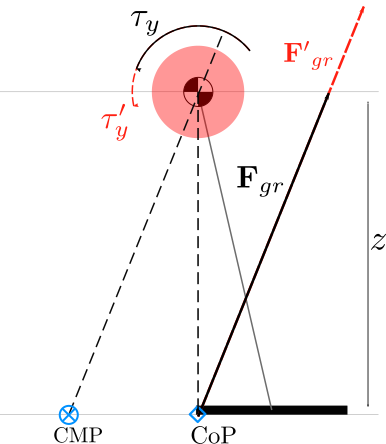
\includegraphics[width=.8\linewidth]{STYLESTUFF/2DCMPVIZCoPzero.png}
  \caption{}
   \label{fig:cmpFzb}
  \end{subfigure}
  \begin{subfigure}{0.36\textwidth}
    \centering
  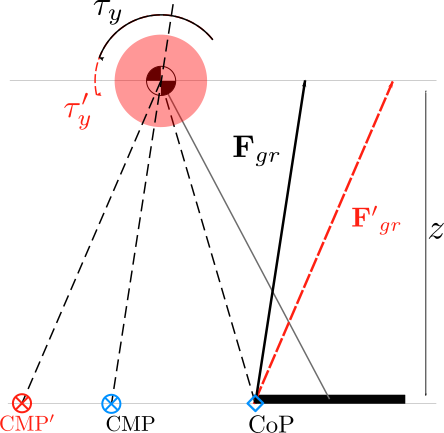
\includegraphics[width=.8\linewidth]{STYLESTUFF/2DCMPVIZFgradjusted.png}
    \caption{}
     \label{fig:cmpFzc}
  \end{subfigure}
  \caption{Effects of change in ground reaction force on angular momentum around the \ac{CoM}. (a) $F_x$ can be scaled up with $F_z$, which results in an increase in $\tau_y$. (b) Situation where additional $F_z$ does not contribute to additional $F_x$. (c) With a shifted \ac{CMP}, a larger $F_x$ can be achieved than with the strategy in (a). }
  \label{fig:cmpFz}
\end{figure}
\subsection{From 2D to 3D}
Direction of desired force can be out of plane with virtual leg between \ac{CoM} and \ac{CoP}. Only one input, $F_z$, can be used to control errors in two directions: $x$ and $y$. If the direction of the desired force is orthogonal to the virtual leg, $F_z$ has no effect. If $F_z$ is increased in one direction, the unstable eigenvalue of the system in the other direction grows. 
\subsection{Leg Reachability}
Stance leg and swing leg singularity need to be avoided. Also, to let the swing leg touch down at the desired time, the ground must be reachable at that time instance. 
\subsection{Predictability of Dynamics}
Considering the current error, is the motion recoverable considering the constraints?
% Experimental Setup
\section{Experimental Setup}
Atlas or Valkyrie walking over a terrain with limited foot placement options, so step adjustment is not possible (tiled environment). Push recovery to test disturbance rejection. See \tabref{tab:stepping} for the used parameters.
\begin{table}[ht]
\caption{Stepping Parameters} % title of Table
\centering % used for centering table
\begin{tabular}{c c c } % centered columns (4 columns)
\hline\hline %inserts double horizontal lines
Parameter & Value & Unit \\
%heading
\hline % inserts single horizontal line
Step Legth & 0.5 &  [m]\\
Step Width & 0.25 & [m]\\
\acs{SS} Time & 0.6 & [s]\\
\acs{DS} Time & 0.15 & [s]\\
%[1ex] % [1ex] adds vertical space
\hline %inserts single line
\end{tabular}
\label{tab:stepping} % is used to refer this table in the text
\end{table}

% Methods
\section{Methods}
Other publications that consider \ac{CoM} height variations for balance use \ac{MPC}. Considering worst-case scenario's, where additional horizontal force is needed, `the best you can do' is needed to not fall over. This motivates to use a proportional controller in worst case scenario's, next to the benefit of simplicity and robustness.
\subsection{Quadratic Program Setup}
One method: use lower weight on vertical momentum rate. To avoid singularity, a feedback based on a virtual spring, priviliged joint accelerations can be projected in the null-space. 
\subsection{Quadratic Program Inputs}
\subsubsection{Control Architecture}
To actively change the desired momentum rate, the effects of additional height acceleration is included in the control framework as follows. 
Horizontal linear momentum rate formula in terms of \ac{CMP}:
\begin{equation}
\dot{\mathbf{l}}_d=\frac{\mathbf{c}_{xy}-\mathbf{r}_{cmp,d}}{z}F_z
\end{equation}
Horizontal linear momentum rate formula in terms of \ac{CoP}:
\begin{equation}
\dot{\mathbf{l}}_d=\frac{\mathbf{c}_{xy}-(\mathbf{r}_{cop,d}+\frac{\tau_y}{F_z})}{z}F_z
\end{equation}
\begin{equation}
\dot{\mathbf{l}}_d=\frac{\mathbf{c}_{xy}-\mathbf{r}_{cop,d}}{z}m(g+\ddot{z}_d) - \frac{\tau_y}{z}
\end{equation}
 This can be written as:
 \begin{equation}
\dot{\mathbf{l}}_d=\underbrace{ \frac{\mathbf{c}_{xy}-\mathbf{r}_{cmp,d}} {z}mg}_{\dot{\mathbf{l}}_{d,lip}}  + \underbrace{\frac{\mathbf{c}_{xy}-\mathbf{r}_{cop,d}}{z}m\ddot{z}_d}_{\dot{\mathbf{l}}_{d,heightcontrol}},
\end{equation}
where $\dot{\mathbf{l}}_{d,lip}$ is the standard desired horizontal momentum rate term and $\dot{\mathbf{l}}_{d,heightcontrol}$ is the additional momentum rate from height control.
\subsubsection{Control Strategy}
If the following criteria are met:
\begin{enumerate}
	\item the desired \ac{CMP} is a certain distance outside the foot polygon
	\item a height or singularity constraint is not met
	\item the angle between the ICP error and the virtual leg between \ac{CoP} and \ac{CoM} in the $xy$ transverse plane is not larger than a specifice value.
\end{enumerate}
ramp up the desired height acceleration with a constant maximum jerk, until the maximum acceleration is reached. Then hold this maximum acceleration, until one of the criteria does not hold anymore. \\
As the strategy is only used when the \ac{CMP} is outside the foot polygon, an estimate of the resulting \ac{CoP} is made by projecting the desired \ac{CMP} on the foot polygon.\\
\figref{fig:3foot} shows initial and final \ac{CoM} and \ac{ICP} configurations for \ac{SS}. \figref{fig:phiViz} shows different alignment angles for the initial configuration, when entering \ac{SS}.\\
\figref{fig:profile} shows an example of a resulting control profile.

\begin{figure}[h]
\centering
  \includegraphics[width=.8\linewidth]{STYLESTUFF/controlProfileConditional.png}
   \caption{Resulting control profile after a push at start of \ac{SS}}
    \label{fig:profile}
\end{figure}

\begin{figure}[h]
\centering
  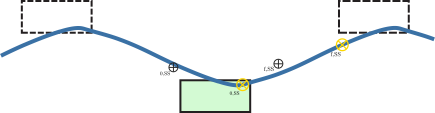
\includegraphics[width=.8\linewidth]{STYLESTUFF/ICPplan3StepComICPrSS.png}
   \caption{Initial (0,SS) and final (f,SS) configurations of \ac{CoM} position (black circle with cross) and \ac{ICP} reference (yellow circle with rotated cross) for \ac{SS} in the $xy$-plane with the parameters from Table \tabref{tab:stepping}. The green area is the current supporting foothold and the blue line is the \ac{ICP} reference trajectory.}
    \label{fig:3foot}
\end{figure}


\begin{figure}[h]
  \begin{subfigure}{0.5\textwidth}
  \centering
  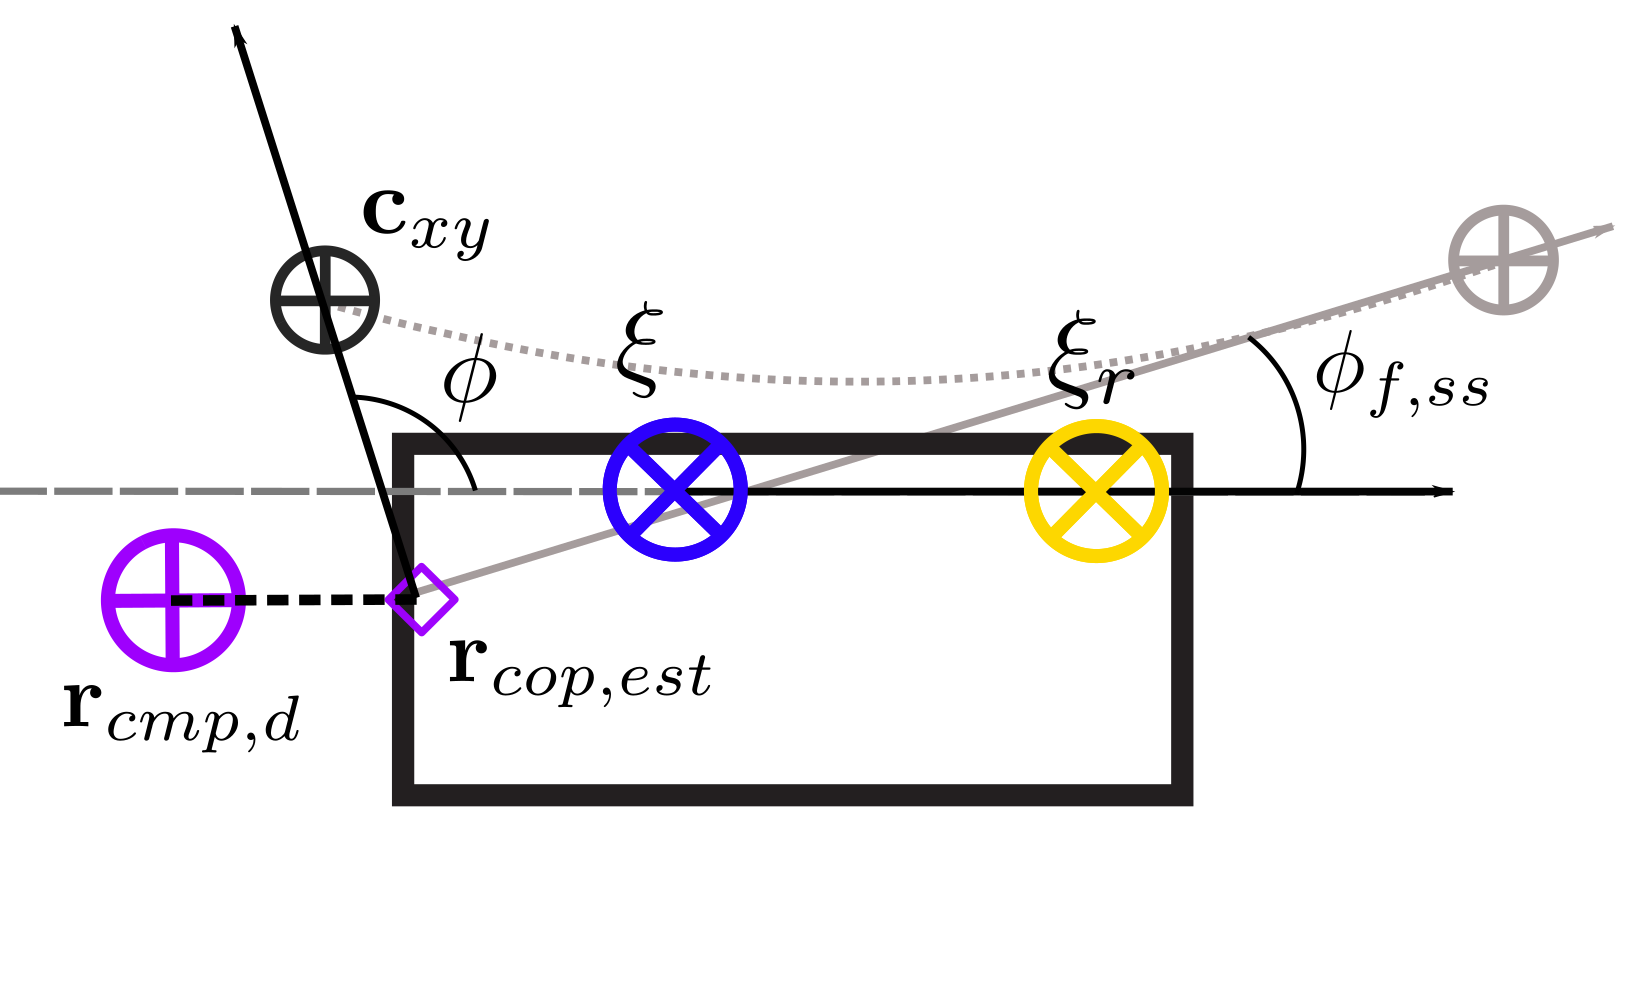
\includegraphics[width=.8\linewidth]{STYLESTUFF/ICPplanStartSSPhiViz.png}
   \caption{}
    \label{fig:phiViza}
  \end{subfigure}
  \begin{subfigure}{0.5\textwidth}
    \centering
  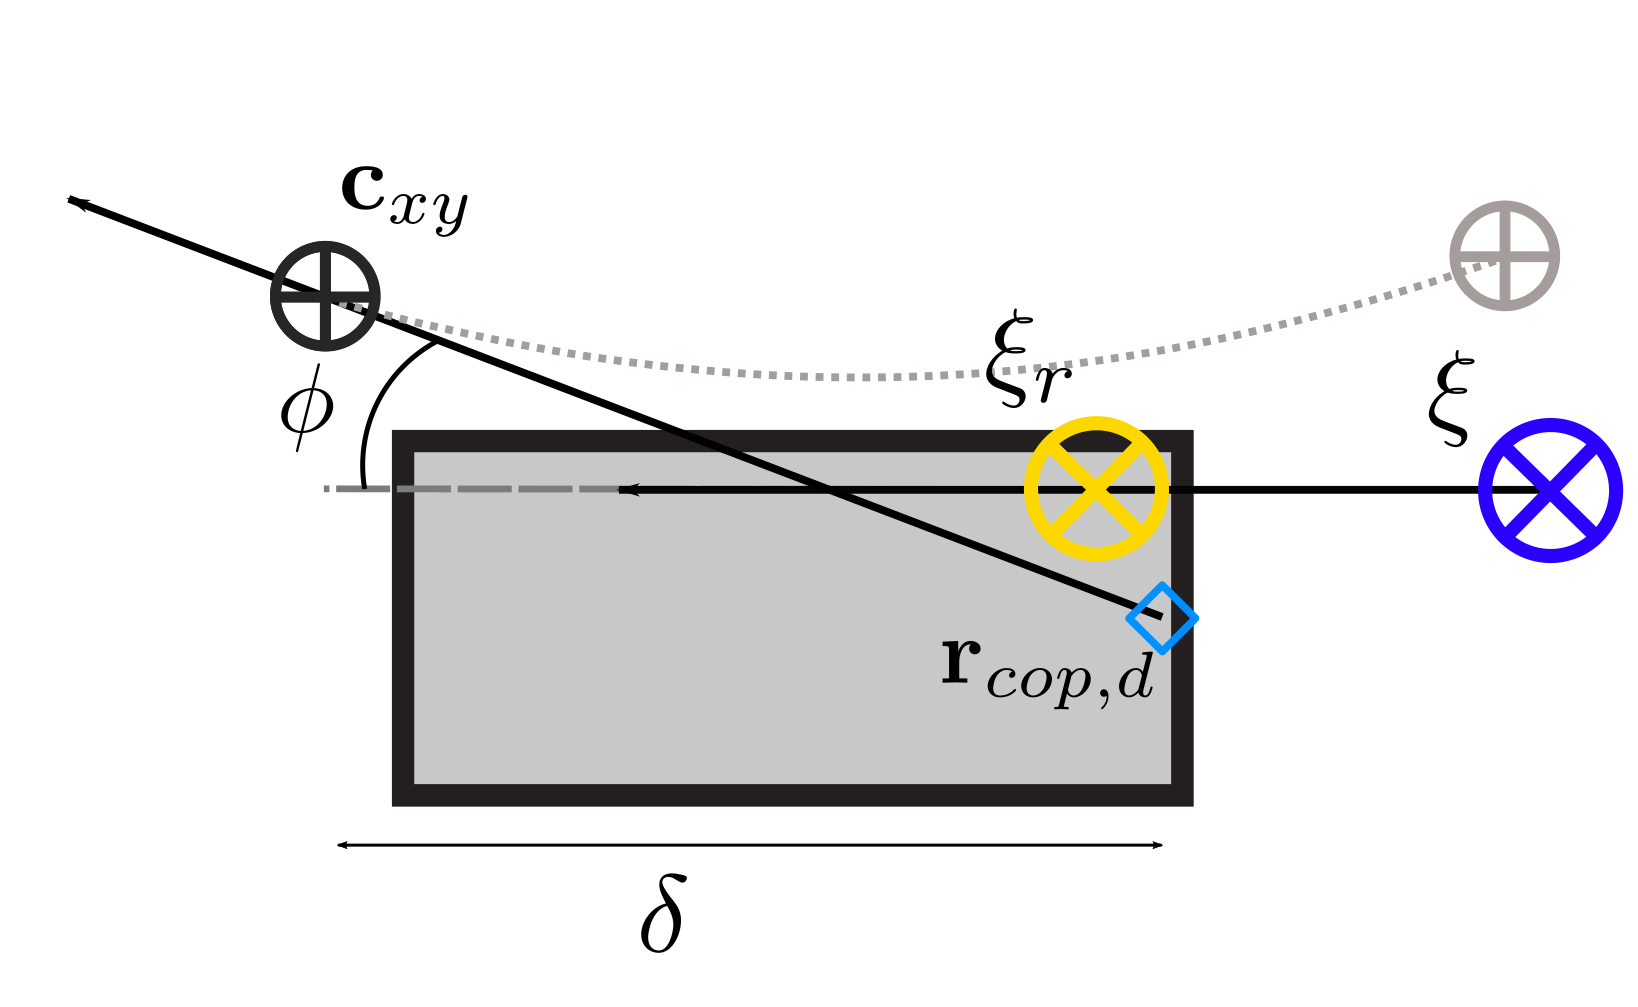
\includegraphics[width=.8\linewidth]{STYLESTUFF/ICPplanStartSSPhiVizNegError.png}
  \caption{}
   \label{fig:phiVizb}
  \end{subfigure}
  \begin{subfigure}{0.5\textwidth}
    \centering
  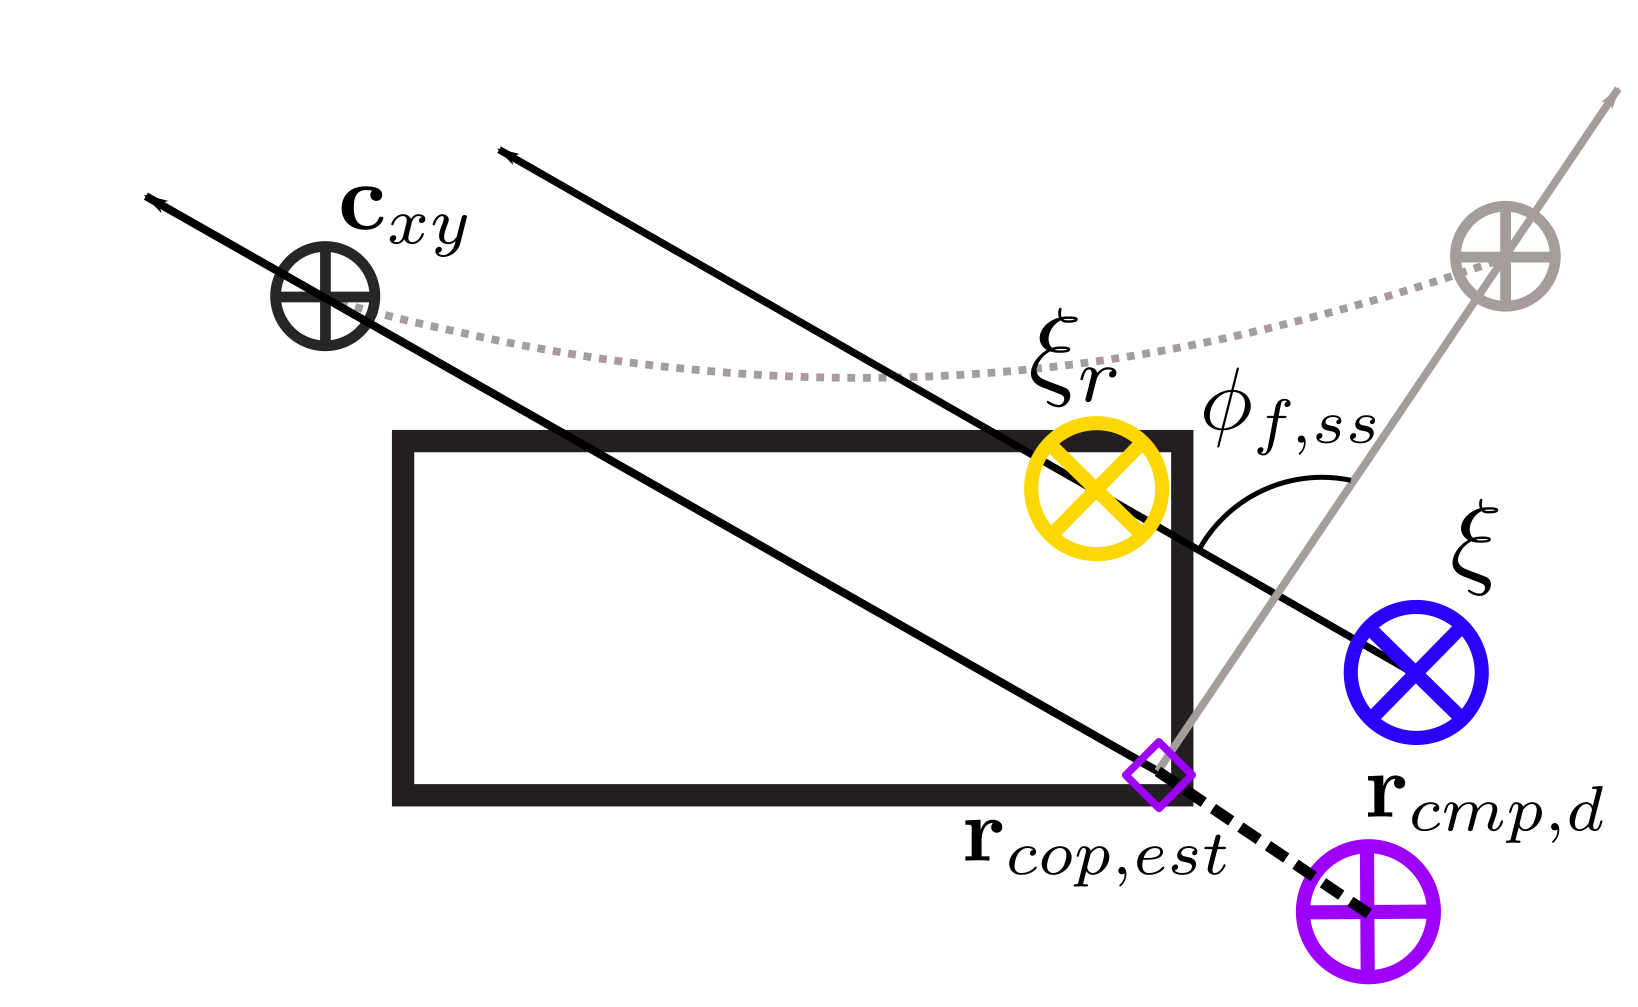
\includegraphics[width=.8\linewidth]{STYLESTUFF/ICPplanStartSSPhiViz0.png}
    \caption{}
     \label{fig:phiVizc}
  \end{subfigure}
  \begin{subfigure}{0.5\textwidth}
    \centering
  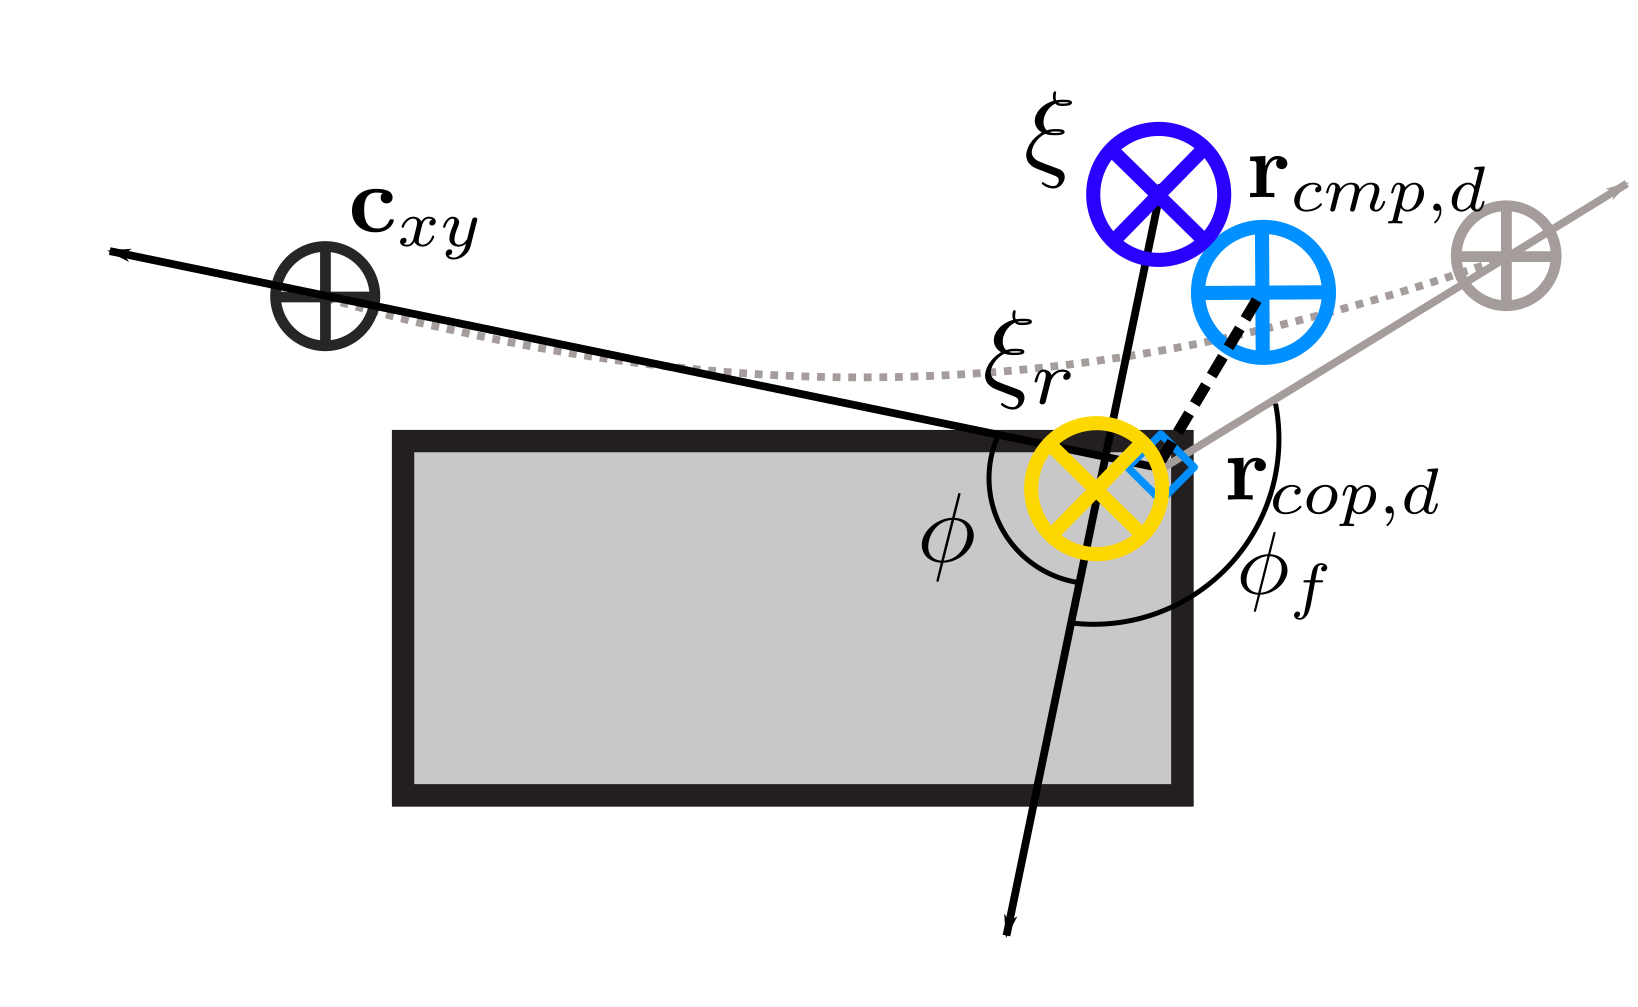
\includegraphics[width=.8\linewidth]{STYLESTUFF/ICPplanStartSSPhiViz90.png}
    \caption{}
     \label{fig:phiVizd}
  \end{subfigure}
  \caption{Vizualizations of the error alignment angle for the configuration at start of \ac{SS}, with \ac{ICP} errors: (a) negative in sagital plane, (b) positive in sagital plane, (c) where the error alignment angle is $0$ and (d) where the error alignment angle is orthogonal to the \ac{ICP} error. }
  \label{fig:phiViz}
\end{figure}


% Results
\section{Results}
\subsection{Simulation}
Comparison with `normal' control setup. (and comparison with `ankle' and `hip' strategies)
\subsection{Hardware}

% Discussion
\section{Discussion}
